\section{Lanford windows}

The time $T^*$ of Theorem~\ref{thm:lanford} is the precise boundary of what the classical proof achieves and the reason a long time theory was needed. We call $[0,T^*]$ a Lanford window. Its existence and size follow from an abstract Cauchy Kovalevskaya argument in a scale of Banach spaces.

\begin{lemma}[Abstract Cauchy Kovalevskaya]
\label{lem:cauchy_kovalevskaya}
Let $(X_r)_{0<r\leq r_0}$ be Banach spaces with $X_r\subset X_{r'}$ and $\|\cdot\|_{r'}\leq\|\cdot\|_r$ for $r'<r$. For each $t\geq0$ let $A(t)$ be a linear operator that maps $X_r$ into $X_{r'}$ for $r'<r\leq r_0$, with $t\mapsto A(t)u$ continuous into $X_{r'}$ for $u\in X_r$, and such that, for all $t\geq0$ and all $r'<r\leq r_0$,
\[
\|A(t)u\|_{r'}\leq\frac{K}{r-r'}\,\|u\|_r.
\]
Then for $u_0\in X_{r_0}$ and $0<r<r_0$ the series
\[
u(t) = \sum_{k\geq0}\int_{0<t_k<\dots<t_1<t}A(t_1)\cdots A(t_k)u_0\dd t_k\cdots\dd t_1
\]
converges in $X_r$ for $0\leq t<T_r = \frac{r_0-r}{eK}$, and it solves $u' = A(t)u$ with $u(0) = u_0$ there, with values in $X_{r'}$ for every $r'<r$.
\end{lemma}

\begin{proof}
Fix $k\geq1$ and split $[r,r_0]$ into $k$ equal intervals of length $\delta/k$, $\delta = r_0-r$. Applying the hypothesis $k$ times, each time losing $\delta/k$,
\[
\|A(t_1)\cdots A(t_k)u_0\|_r\leq\Big(\frac{Kk}{\delta}\Big)^k\|u_0\|_{r_0}\qquad\text{for all }t_1,\dots,t_k.
\]
The simplex $0<t_k<\dots<t_1<t$ has volume $t^k/k!$, and $k^k\leq e^kk!$, so the $k$th term $u_k(t)$ of the series satisfies $\|u_k(t)\|_r\leq\big(\frac{eKt}{\delta}\big)^k\|u_0\|_{r_0}$, a geometric series that converges for $t<\delta/(eK)$. Since $u_k(t) = \int_0^tA(s)u_{k-1}(s)\dd s$ and $\|A(s)u_{k-1}(s)\|_{r'}\leq\frac{K}{r-r'}\|u_{k-1}(s)\|_r$ for $r'<r$, the series $\sum_kA(s)u_{k-1}(s)$ converges in $X_{r'}$ locally uniformly in $s<T_r$. Hence $u(t) = u_0+\int_0^tA(s)u(s)\dd s$ in $X_{r'}$, which is the equation.
\end{proof}

Lanford applies the lemma to the BBGKY and Boltzmann hierarchies with the scale of norms
\[
\|F\|_{\beta,\gamma} = \sup_{s\geq1}\sup_{Z_s}e^{\gamma s}\,e^{\beta E(Z_s)}\,|F^{(s)}(Z_s)|,\qquad E(Z_s) = \frac12\sum_{i\leq s}|v_i|^2,
\]
which measure Gaussian decay in velocity and exponential decay in the number of particles. The generator of each hierarchy contains the free transport, which is unbounded in these norms, and one passes to the interaction picture. The free flow $S(t)$ preserves $E(Z_s)$ and is therefore an isometry of $\|\cdot\|_{\beta,\gamma}$, so $u(t) = S(-t)F(t)$ solves $u' = A(t)u$ with $A(t) = S(-t)\,C\,S(t)$, where $C$ collects the collision operators $C_{s,s+1}$, and the series of the lemma is the Duhamel series of the hierarchy. The collision operator $C_{s,s+1}$ integrates over the velocity of the added particle and multiplies by a relative velocity, so it costs one factor $\beta^{-d/2}$ from the Gaussian integral, one factor of $s$ from the sum over particles, and one factor $\sum_{i\leq s}|v_i|+|v_{s+1}|$ from the cross section. The factors of $s$ and of velocity are absorbed by giving up a little decay: since $s\,e^{-\eta s}\leq(e\eta)^{-1}$ and $\sum_i|v_i|\,e^{-\eta E}\leq C\sqrt{s/\eta}$, decreasing $\gamma$ and $\beta$ by amounts proportional to $r-r'$ along a fixed line in the $(\beta,\gamma)$ plane produces exactly the hypothesis of the lemma, with $K$ proportional to $\alpha\beta^{-d/2}$ times a function of $(\beta,\gamma)$. The lemma then gives a window
\[
T^* = \frac{r_0-r}{eK}\;\asymp\;c_d\,\tau_{\mathrm{mf}},
\]
a fixed fraction of the mean free time $\tau_{\mathrm{mf}}\asymp(\alpha\langle|v|\rangle)^{-1}$, independent of $N$. Figure~\ref{fig:lanford} is a schematic of the mechanism.

\begin{figure}[t]
\centering
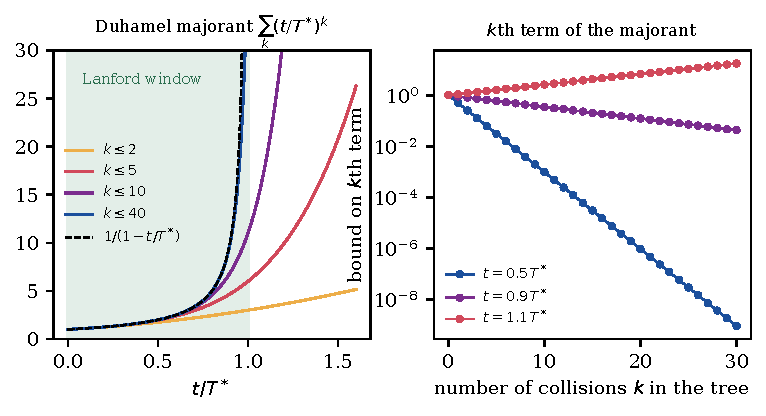
\includegraphics[width=\textwidth]{lanford_window}
\caption{Schematic of the Lanford window. Left, partial sums of the majorant $\sum_k(t/T^*)^k$ of the Duhamel series converge for $t<T^*$ (shaded) to the limit $1/(1-t/T^*)$, drawn dashed, and diverge beyond. Right, the $k$th term $(t/T^*)^k$ of the majorant, a bound on the contribution of collision trees with $k$ branchings, for $t = 0.5\,T^*$, $0.9\,T^*$ and $1.1\,T^*$: it decays geometrically inside the window and grows outside. No hard sphere quantity is computed.}
\label{fig:lanford}
\end{figure}

\subsection{Why windows cannot simply be iterated}

If chaos at time zero implies chaos at time $T^*$, why not restart the argument at $T^*$ and cover any interval by finitely many windows? The obstruction is that the conclusion of the theorem is weaker than its hypothesis. At time zero the $N$ particle law is a product measure restricted to the hard sphere phase space, with bounds in the norm $\|\cdot\|_{\beta,\gamma}$. At time $T^*$ the limit is again a product, but at finite $N$ the law carries correlations created by collisions, of size $O(\varepsilon)$ in a weak sense but not small in the norms the lemma requires, and the decay parameters have been spent: the window was obtained by trading $(\beta_0,\gamma_0)$ for $(\beta,\gamma)$, and the next window would start from worse parameters. A naive iteration therefore produces a sequence of windows whose lengths sum to a finite total.

Three ways around the obstruction are known. At equilibrium the Gibbs measure is invariant, so the a priori bounds at time $T^*$ are as good as at time zero, and many windows can be concatenated. Bodineau, Gallagher, Saint Raymond and Simonella use this invariance, for a gas in a periodic box in dimension at least three, first to show that the covariance of the fluctuations of the empirical measure is governed by the linearized Boltzmann equation globally in time, by a duality method combined with a pruning of the collision trees that removes those with superexponential growth~\cite{bgss2023cpam}, and then to show that the whole fluctuation field converges, for all times, to the solution of the fluctuating Boltzmann equation, by a study of clusters of pseudo trajectories, with quantitative bounds on time intervals that grow, slowly, with the number of particles~\cite{bgss2024}. Away from equilibrium the same authors control fluctuations and large deviations of the empirical measure, but only for short times~\cite{bgss2023}. Near equilibrium, a refinement of Lanford's argument based on estimates of the pathological collision trees gives the Brownian motion of a tagged particle of Chapter~\ref{ch:brownian}, in a diffusive limit~\cite{bgs2016}. Far from equilibrium, Deng, Hani and Ma do iterate short windows, which they call time layers, but they propagate across the layers a cumulant ansatz that records the correlations created in the earlier layers~\cite{denghanima2024}, as described after Theorem~\ref{thm:dhm}.

\subsection{Moment conditioning inside the window}

The initial data of Theorem~\ref{thm:lanford} are products restricted to non overlapping configurations, not data conditioned on moments, and what follows is a heuristic and not a theorem. A gas prepared with prescribed local density, velocity and temperature is, in the language of Chapter~\ref{ch:types}, a large system conditioned on local moments, and the conditional limit theorem suggests that its $k$ particle marginals are close to products of local Maxwellians. Lanford's theorem propagates a product structure for the length of a window, and the $H$ theorem (Theorem~\ref{thm:htheorem}) describes how the one particle law then relaxes toward the Maxwellian determined by the conserved moments. On this reading the passage from atoms to continua has three steps: conditioning on moments produces chaos, Lanford windows propagate chaos, and the Hilbert expansion of Chapter~\ref{ch:hydro} reads off the evolution of the conditioned moments as the equations of fluid dynamics. The three step picture is our framing of the subject: the first step is the heuristic above, and the second and third are Theorems~\ref{thm:lanford} and~\ref{thm:dhm} and the hydrodynamic limits of Chapter~\ref{ch:hydro}.
